\documentclass[11pt,a4paper]{article}

\usepackage[margin=1in]{geometry}
\usepackage[T1]{fontenc}
\usepackage[utf8]{inputenc}
\usepackage{array}
\usepackage{booktabs}
\usepackage{graphicx}
\usepackage{hyperref}
\usepackage{longtable}
\usepackage{parskip}
\usepackage{tabularx}
\usepackage{xcolor}

\hypersetup{
  colorlinks=true,
  linkcolor=blue!50!black,
  urlcolor=blue!50!black
}

\title{Task 1 Opponent Vehicle Detection\\Engineering Challenge 2026}
\author{mesa-ec2026-av-challenge}
\date{\today}

\begin{document}
\maketitle

\begin{abstract}
This report explains the complete first-pass Task 1 pipeline implemented for
opponent vehicle detection. The pipeline inspects the ROS 2 bag metadata, selects
a supported point-cloud topic, reads only a limited number of frames, converts
the point cloud into a bird's-eye-view (BEV) representation, clusters candidate
objects, filters clusters using vehicle-like constraints, writes detections to a
CSV file, and saves BEV visualizations. The current run processed 20 frames from
\path{/sensor/lidar_front/points} and produced 99 candidate opponent detections.
\end{abstract}

\section{Challenge Goal}

Task 1 asks us to detect opponent vehicles using one or more sensors. The
expected output is:

\begin{itemize}
  \item target positions,
  \item bounding boxes or cluster detections,
  \item visualizations of detected targets.
\end{itemize}

The challenge evaluation criteria are accuracy, robustness, and false positive
reduction. The current repository does not include ground-truth opponent labels,
so this report separates what can be measured now from what needs labelled data.

\section{Input Data}

The ROS 2 bag is stored as sqlite3 database files in the \path{data/} directory:

\begin{longtable}{p{0.38\linewidth}rrp{0.27\linewidth}}
\toprule
Storage file & Duration & Size & Start time \\
\midrule
\path{2025-10-08_09-35_sensors_raw_0.db3} & 119.950 s & 12.80 GiB & 2025-10-08T05:45:45.780411+00:00 \\
\path{2025-10-08_09-35_sensors_raw_1.db3} & 119.906 s & 13.77 GiB & 2025-10-08T05:47:45.823226+00:00 \\
\bottomrule
\end{longtable}

The full bag duration is 239.949 s, or about four minutes. The files look large
because the bag contains raw high-throughput sensors: multiple compressed
cameras, three LiDAR point clouds, four radar point clouds, and transform
messages. The storage files are chunks of the same recording, not separate long
sessions.

\section{Discovered Topics}

The code does not assume topic names. It first reads \path{metadata.yaml} and
prints a readable summary. The relevant point-cloud topics discovered were:

\begin{longtable}{p{0.43\linewidth}p{0.32\linewidth}r}
\toprule
Topic & Message type & Messages \\
\midrule
\path{/sensor/lidar_front/points} & \path{sensor_msgs/msg/PointCloud2} & 4800 \\
\path{/sensor/lidar_left/points} & \path{sensor_msgs/msg/PointCloud2} & 4799 \\
\path{/sensor/lidar_right/points} & \path{sensor_msgs/msg/PointCloud2} & 4800 \\
\path{/sensor/radar_front/points} & \path{sensor_msgs/msg/PointCloud2} & 3999 \\
\path{/sensor/radar_left/points} & \path{sensor_msgs/msg/PointCloud2} & 4000 \\
\path{/sensor/radar_right/points} & \path{sensor_msgs/msg/PointCloud2} & 4000 \\
\path{/sensor/radar_back/points} & \path{sensor_msgs/msg/PointCloud2} & 4000 \\
\bottomrule
\end{longtable}

Because standard \path{sensor_msgs/msg/PointCloud2} topics were available, the
pipeline could parse the bag without installing a full ROS 2 environment. It uses
sqlite3 for storage access and \path{rosbags} for CDR deserialization.

\section{Implemented Pipeline}

The implementation is split into the following files:

\begin{itemize}
  \item \path{src/bag_inspector.py}: reads \path{metadata.yaml}, summarizes
  duration, storage files, topics, message types, and counts.
  \item \path{src/task1_detection.py}: reads PointCloud2 frames, converts points
  to BEV coordinates, clusters points, filters candidate vehicles, and writes
  outputs.
  \item \path{src/visualization.py}: saves BEV plots with raw points and bounding
  boxes.
  \item \path{scripts/run_task1.py}: command-line entry point.
\end{itemize}

The command used for the current run was:

\begin{verbatim}
uv run python scripts/run_task1.py --bag-dir data --max-frames 20 --output-dir outputs/task1
\end{verbatim}

\subsection{Topic Selection}

If no topic is supplied through \path{--topic}, the detector prefers front LiDAR
when present. For this run it selected:

\begin{center}
\path{/sensor/lidar_front/points}
\end{center}

This topic contains standard PointCloud2 data, so no custom message support was
needed.

\subsection{Frame Limiting}

The bag is large, so the detector intentionally avoids loading the entire
dataset into memory. It iterates through sqlite rows for the selected topic and
stops after \path{--max-frames}. The current run used 20 frames.

\subsection{PointCloud2 Parsing}

Each PointCloud2 message is converted into a structured NumPy array using the
field metadata from the message. The front LiDAR fields include:

\begin{center}
\path{x}, \path{y}, \path{z}, \path{timestamp}, \path{intensity},
\path{scan_idx}, \path{scan_id}, \path{ring}, \path{channel}.
\end{center}

The point cloud layout in this bag uses:

\begin{itemize}
  \item \path{z} as forward range,
  \item \path{x} as lateral position,
  \item \path{y} as the vertical-like axis.
\end{itemize}

Therefore the BEV point used for clustering is:

\[
  p_{\mathrm{BEV}} = \left[z, x\right]
\]

In the output CSV these are named \path{center_x} for forward position and
\path{center_y} for lateral position.

\subsection{Cropping and Noise Reduction}

Before clustering, points are cropped to a racing-relevant region:

\[
  3.0 \leq x_{\mathrm{forward}} \leq 95.0 \quad\mathrm{m}
\]

\[
  -18.0 \leq y_{\mathrm{lateral}} \leq 18.0 \quad\mathrm{m}
\]

The detector also applies a simple ground-band filter when possible. This filter
uses nearby points to estimate a median vertical band and removes points very
close to that band. This is a conservative first-pass way to reduce ground
returns before DBSCAN.

\subsection{Clustering}

The detector runs DBSCAN on the BEV points. For LiDAR, the current settings are:

\begin{itemize}
  \item DBSCAN radius: \path{eps = 0.45},
  \item minimum samples: \path{min_samples = 6},
  \item minimum retained LiDAR points per detection: 15.
\end{itemize}

DBSCAN groups nearby points without requiring us to know the number of opponent
vehicles in advance.

\subsection{Vehicle Candidate Filtering}

After clustering, each cluster is converted into an axis-aligned BEV bounding
box:

\[
  \mathrm{length} = \max(x) - \min(x)
\]

\[
  \mathrm{width} = \max(y) - \min(y)
\]

The current plausible vehicle footprint filter keeps clusters satisfying:

\[
  0.8 \leq \mathrm{width} \leq 4.8 \quad\mathrm{m}
\]

\[
  1.2 \leq \mathrm{length} \leq 9.0 \quad\mathrm{m}
\]

These thresholds reduce obvious false positives such as tiny noise groups,
extremely thin structures, and very large non-vehicle surfaces.

\section{Detection Output}

The main result file is:

\begin{center}
\path{outputs/task1/detections.csv}
\end{center}

Each row represents one candidate opponent detection. The columns are:

\begin{longtable}{p{0.25\linewidth}p{0.65\linewidth}}
\toprule
Column & Meaning \\
\midrule
\path{timestamp} & ROS bag timestamp in nanoseconds. \\
\path{topic} & Sensor topic used for the detection. \\
\path{source_frame} & Source sensor frame, here \path{lidar_front}. \\
\path{frame_index} & Local processed-frame index. \\
\path{detection_id} & Unique ID within the processed run. \\
\path{center_x}, \path{center_y} & BEV center position: forward and lateral meters. \\
\path{width}, \path{length} & Axis-aligned BEV cluster size in meters. \\
\path{min_x}, \path{max_x}, \path{min_y}, \path{max_y} & BEV bounding box limits. \\
\path{point_count} & Number of points in the retained cluster. \\
\path{confidence} & Heuristic score based on point support, shape plausibility, and range. \\
\bottomrule
\end{longtable}

\subsection{Current Run Results}

\begin{table}[h]
\centering
\begin{tabular}{lr}
\toprule
Metric & Value \\
\midrule
Selected topic & \path{/sensor/lidar_front/points} \\
Frames processed & 20 \\
Total detections & 99 \\
Frames with detections & 20/20 \\
Mean detections per frame & 4.95 \\
Maximum detections in one frame & 8 \\
Mean confidence & 0.666 \\
Median confidence & 0.674 \\
Low-confidence detections below 0.50 & 5 \\
Mean candidate width & 1.53 m \\
Mean candidate length & 3.31 m \\
Mean candidate point count & 74.1 \\
Deserialization failures & 0 \\
\bottomrule
\end{tabular}
\caption{Summary metrics from the 20-frame run.}
\end{table}

The detected candidate centers in this run span approximately 22.91 m to
93.62 m forward and -3.82 m to 5.92 m laterally. This indicates that the current
front-LiDAR baseline is mostly finding candidates in front of the ego vehicle,
which is expected from the selected topic and crop.

\section{Visualization}

The pipeline saves one BEV plot per processed frame in:

\begin{center}
\path{outputs/task1/frame_*.png}
\end{center}

Raw points are shown in gray. Detected candidate clusters are drawn as colored
axis-aligned bounding boxes and labelled with their detection IDs.

\begin{figure}[h]
  \centering
  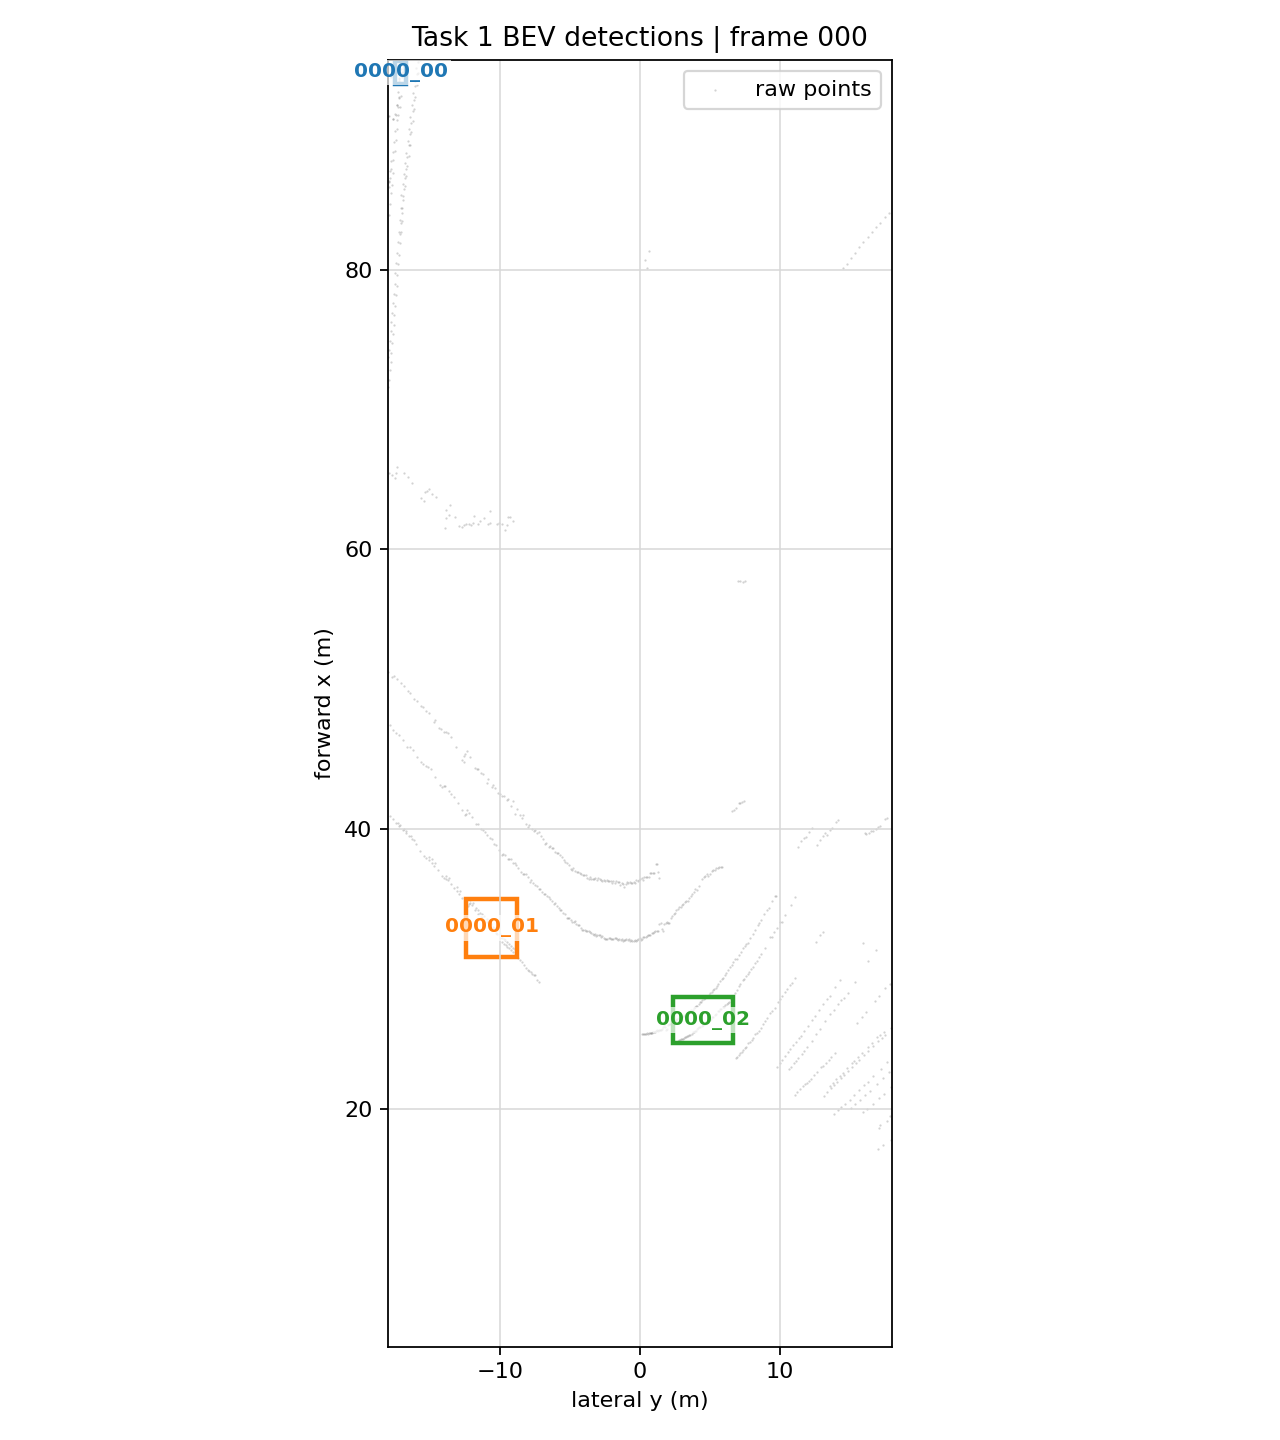
\includegraphics[width=0.68\linewidth]{frame_000.png}
  \caption{BEV detections for frame 000.}
\end{figure}

\begin{figure}[h]
  \centering
  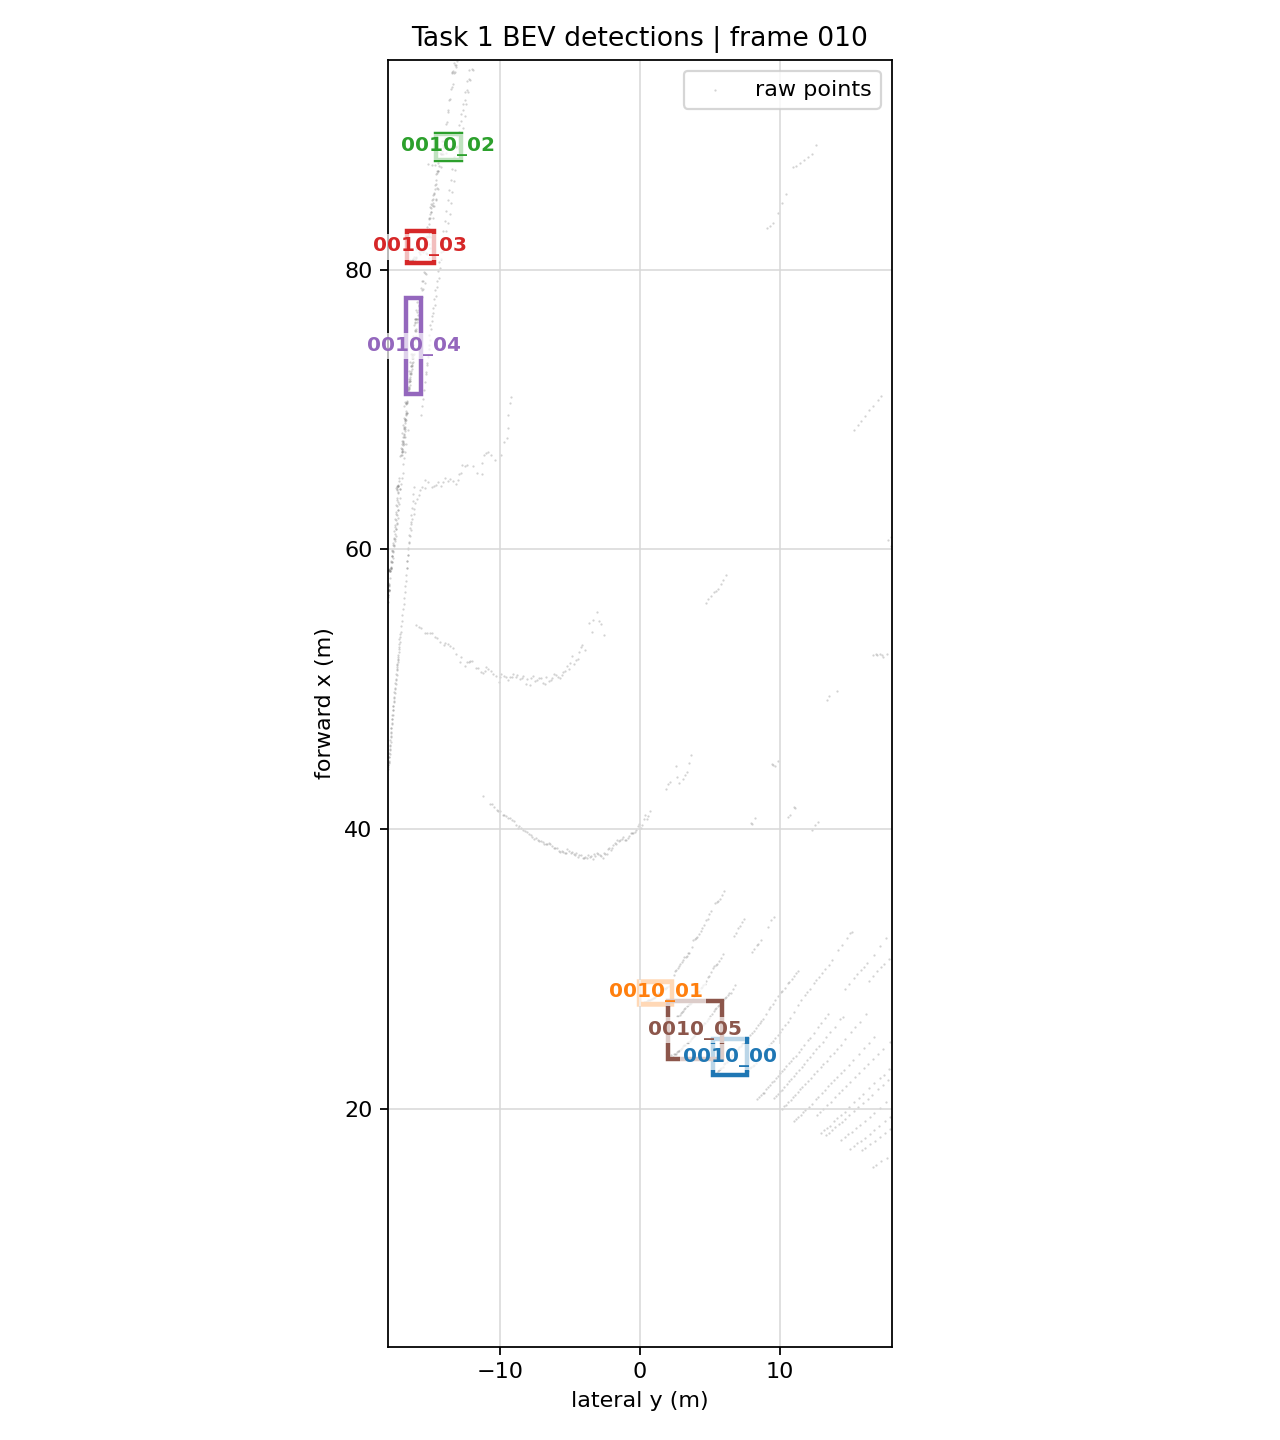
\includegraphics[width=0.68\linewidth]{frame_010.png}
  \caption{BEV detections for frame 010.}
\end{figure}

\section{Evaluation Criteria}

The generated evaluation summary is:

\begin{center}
\path{outputs/task1/evaluation_summary.csv}
\end{center}

\subsection{Accuracy}

The detector produces the required target positions and bounding boxes. However,
the project data currently does not include labelled opponent vehicle positions
or bounding boxes. Because of that, true accuracy metrics such as precision,
recall, center-position error, and intersection-over-union cannot be computed
honestly yet.

What is available now:

\begin{itemize}
  \item 99 candidate detections were generated.
  \item Each detection includes center position, bounding box limits, dimensions,
  point count, and confidence.
  \item BEV plots allow manual inspection of candidate quality.
\end{itemize}

What is needed for real scoring:

\begin{itemize}
  \item ground-truth opponent center positions, or
  \item ground-truth opponent bounding boxes in the same BEV frame, or
  \item a transformation/calibration path from labelled world coordinates into
  the selected sensor frame.
\end{itemize}

\subsection{Robustness}

The run processed 20 frames without reading the full 26.58 GiB bag into memory.
There were no PointCloud2 deserialization failures. Every processed frame had at
least one retained candidate. This is a basic robustness signal: the pipeline can
iterate through real bag messages, parse them, and produce stable outputs over a
limited window.

\subsection{False Positive Reduction}

False positives are reduced through several filters:

\begin{itemize}
  \item spatial crop to the useful forward/lateral racing region,
  \item vertical outlier trimming,
  \item optional ground-band removal,
  \item DBSCAN minimum support,
  \item vehicle-like width and length constraints,
  \item confidence score for ranking detections during review.
\end{itemize}

These are proxy controls. The final false-positive rate still requires labelled
negative/positive examples.

\section{Limitations and Next Steps}

This report describes a smallest working baseline, not a final competition-grade
detector. The current limitations are:

\begin{itemize}
  \item only one PointCloud2 topic is processed at a time,
  \item LiDAR/radar/camera fusion is not implemented yet,
  \item sensor extrinsic calibration is not applied,
  \item boxes are axis-aligned in BEV rather than oriented,
  \item confidence is heuristic,
  \item true quantitative accuracy needs ground truth.
\end{itemize}

Recommended next steps:

\begin{enumerate}
  \item Add ground-truth labels or load the challenge evaluator if provided.
  \item Fuse front, left, and right LiDAR into a common ego frame.
  \item Add temporal tracking so one opponent has a consistent identity across
  frames.
  \item Replace axis-aligned boxes with oriented boxes.
  \item Tune DBSCAN and filtering parameters against labelled validation data.
  \item Compare LiDAR-only, radar-only, and fused detections.
\end{enumerate}

\section{Conclusion}

The implemented Task 1 baseline successfully reads the ROS 2 sqlite bag without
a full ROS 2 installation, discovers the available topics from metadata, parses
standard PointCloud2 LiDAR data, converts points to BEV coordinates, clusters
candidate vehicles, writes detections to CSV, and produces visualizations. For
the current 20-frame run, it generated 99 candidate detections with no
deserialization failures. The report also now explicitly maps the output to the
challenge criteria and states what remains necessary for true accuracy scoring.

\end{document}
